\section{Bewijslast}
Dit hoofdstuk bevat de bewijslast voor de leerdoelen die in het Plan van Aanpak staan. Hier zal een apart hoofdstuk per leerdoel komen waar in diepte wordt uitgelegd waarom dit leerdoel is behaald.

\subsection{Facebook API}

\clearpage

\subsection{Meteor, een JavaScript framework}
Het leerdoel dat hierbij hoort: Meteor leren kennen door middel van een applicatie te maken die real-time informatie weergeeft over een klant’s social media kanalen aan meerdere eind-gebruikers, dit wordt verwezenlijkt door Meteor’s collections en het publish-subscribe pattern te gebruiken.

Normaliter deed ConnectSB alles met PHP en dan vooral het Symfony framework. Profile2Connect was een speciaal geval, het moest mogelijk zijn om heel veel data op te slaan en dynamisch velden toe te voegen aan de database. Door deze speciale eisen is er toen gekozen voor Meteor. Meteor is een JavaScript framework waarmee het mogelijk is om de backend evenals de frontend in JavaScript te programmeren. Meteor is zeer recent, op het moment van schrijven is Meteor nog in beta, versie 0.9.3.1 om precies te zijn. Dit brengt natuurlijk wel de nodige problemen met zich mee, weinig documentatie en vooral veel kans op performance issues. Meteor zelf maakt gebruik van het publish-subscribe pattern om zogenaamde collecties van de server naar de client beschikbaar te maken. Deze collecties zijn niets anders als tabellen, op de server worden ze gepublished en op de client kun je deze dan ontvangen (subscriben). Op de server kun je aangeven welke velden er wel beschikbaar worden gemaakt en welke niet, wegens performance issues is het natuurlijk beter om alleen de velden beschikbaar te maken die nodig zijn.

\newline

Meteor beschikt ook over iets wat heet latency compensation. Als een eind-gebruiker iets veranderd ziet deze eind-gebruiker de verandering meteen. Meteor stuurt dit daarna op, ontvangt de respons, vergelijkt dit met de client en voert daarna de echte wijziging door. De eind-gebruiker ziet hier niets van, tenzij er iets mis gaat in het proces van vergelijken maar dat gebeurt nagenoeg nooit. Met een platform waar heel veel data in staat kan het wel eens zijn dat de database verbinding wat aan de trage kant wordt, Meteor zorgt ervoor dat hoe langzaam de verbinding ook wordt de eind-gebruiker hier maar minimaal mee te maken zal hebben.

\newline

Profile2Connect wordt gemaakt door mij en nog een medewerker van ConnectSB, Jimmy. Ik ben verantwoordeljik voor de homepage van Profile2Connect welke er als volgt uitziet:

\begin{center}
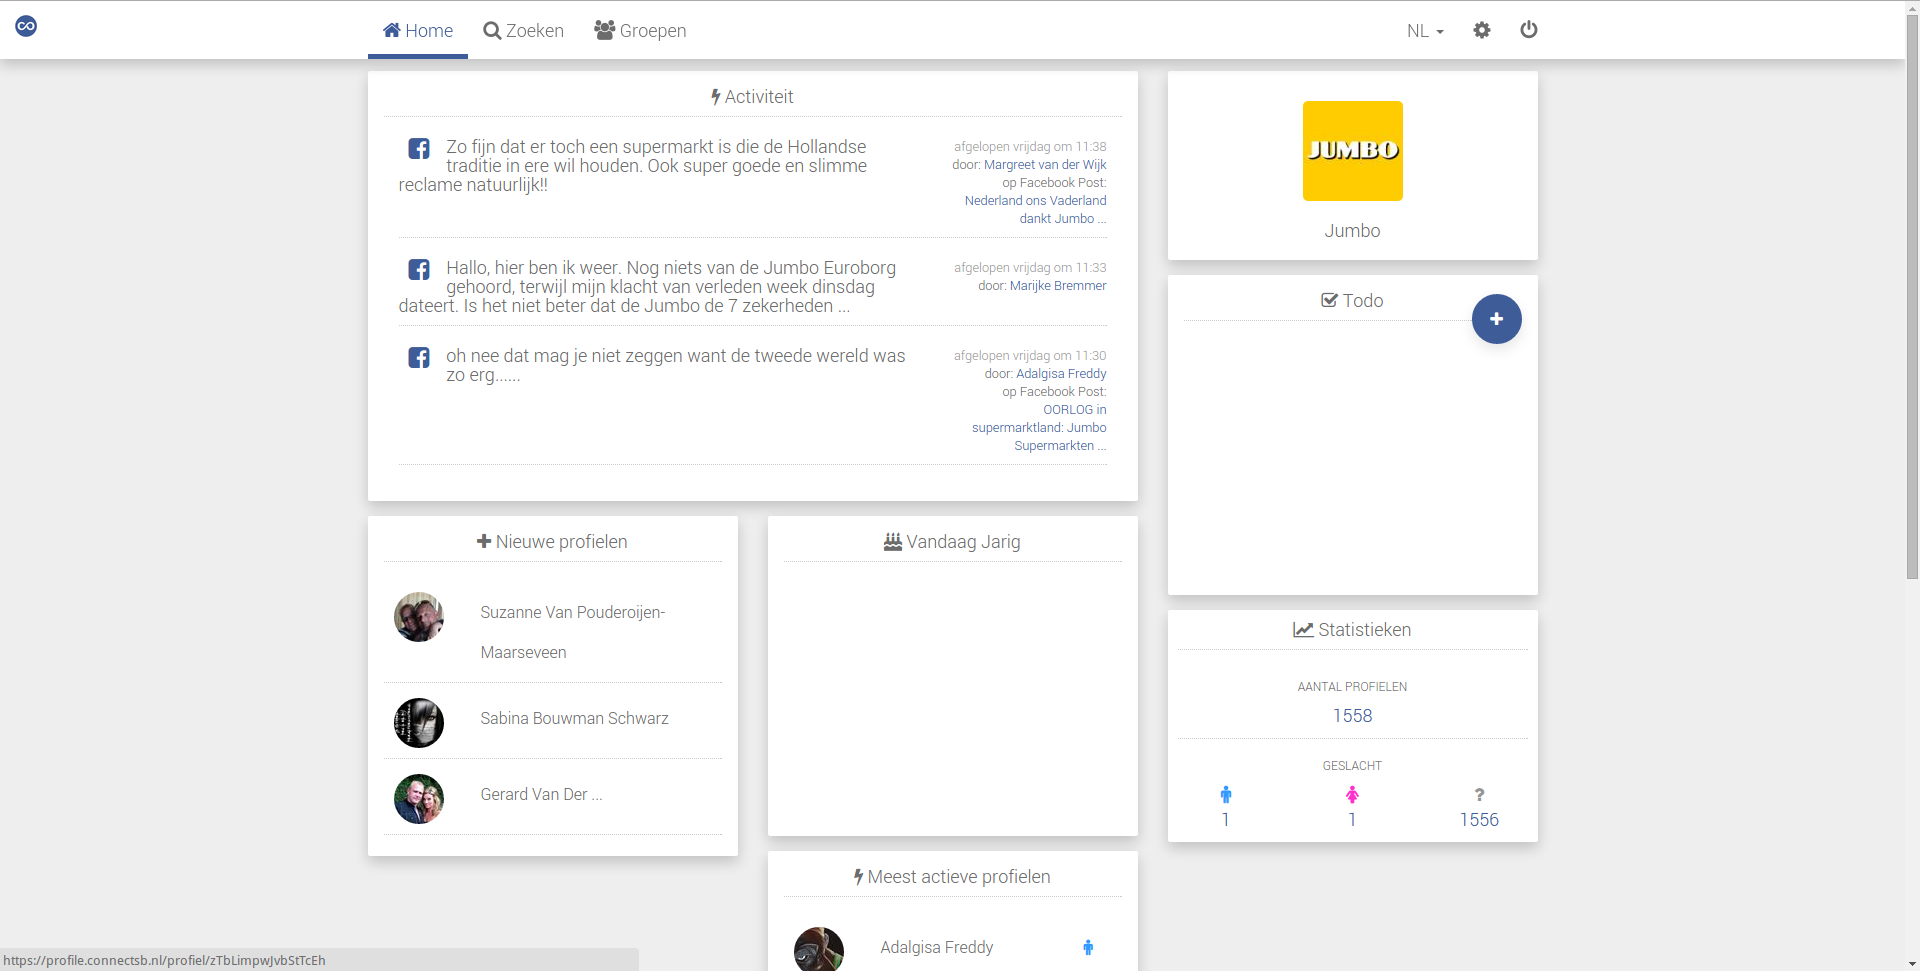
\includegraphics[scale=0.2]{profile2connect}
\end{center}


De gegevens die te zien zijn op deze pagina komen van verschillende publicaties. Zo zie je bijvoorbeeld een logo van de op dit moment ingelogde klant(rechts boven in), de updates (links boven in) en dan nog een aantal overige categoriën zoals nieuwe profielen en meest actieve profielen. Al deze categoriën zijn allemaal aparte publicaties, dit wordt gedaan omdat je dan nooit meer data beschikbaar hebt op de client dan dat je nodig hebt. Het optellen van de totalen wordt ook op de server gedaan, je wilt natuurlijk niet alle profielen van een klant op de welkomst pagina beschikbaar maken. Hierdoor zou de applicatie heel lang kunnen doen over het laden, omdat hij al deze profielen uit de database zou moeten halen.

\clearpage

\subsection{Versiebeheer}
Het desbetreffende leerdoel is: Versiebeheer volgens de Gitflow workflow gebruiken zodat er altijd een fout vrije en uitrolbare versie van de applicatie beschikbaar is en als er een fout optreedt deze snel weer ongedaan gemaakt kan worden door naar een vorige versie terug te keren.

\newline

Voor Content2Connect moesten een aantal belangrijke fixes gebeuren, deze hadden hoge prioriteit. Deze komen volgens de Gitflow workflow dan op zogenaamde feature branches. Er is geen speciale conventie voor hoe deze feature branches moeten heetten maar heel veel bedrijven houden de volgende conventie aan: feature/[feature-naam], dit heb ik dus ook gedaan. Mijn branch voor deze belangrijke fixes heet daarom ook feature/important-fixes. Bij ConnectSB wordt gewerkt met Redmine en hierbij kan er prioriteit gegeven worden aan bepaalde issues. Deze hoge prioriteit komt dus ook van Redmine.

Voor een grote hoeveelheid met kleine issues is het in mijn belevenis beter om een branch te maken die deze allemaal bevat. Veel bedrijven houden zich ook aan het aanmaken van één branch voor elke issue, maar dit is naar mijn idee geen goed idee. Als een issue natuurlijk best wel uitgebreid is en je waarschijnlijk kleine taken zult hebben is dit een goed idee, maar als je één issue moet doen die hooguit 5 minuten duurt is dit het natuurlijk niet echt waard.

\newline

Ik moest in Content2Connect bij het overzicht van één bestelling de titel toevoegen van de bestelling. Hiervoor wordt er dan een branch gemaakt genaamd feature/change-\#2318 want de issue heet op Redmine Change \#2318. Change is dan de categorie en \#2318 is het nummer van de issue.

Dit is dus nu gedaan voor elke issue die op Redmine stond. Deze branches komen eigenlijk nooit op de centrale repository. Deze kunnen gepusht worden als dat nodig is, bijvoorbeeld als iemand mee moet helpen om aan een bepaalde feature mee te werken. Features zullen meest van de tijd, in ieder geval in mijn situatie, werk bevatten voor één persoon dus de feature branches hoeven dan nooit gepusht te worden.

\newline

Vandaag is er een release voor Content2Connect uitgebracht. Dit is versie v0.9, hier wordt dan een tag voor aangemaakt op de master en dan kan deze in productie gezet worden.

Gitflow workflow werkt vooral heel goed als je bijvoorbeeld bezig bent aan nieuwe functionaliteit, maar je baas zegt dat er even snel wat anders moet gebeuren. Je maakt een nieuwe feature branch aan, commit daar alles op. Deze merge je dan met de develop branch en indien nodig kan deze naar master voor een nieuwe release. Alle changes waar je dan eerst mee bezig was kun je dan heel gemakkelijk weer.

\clearpage

\subsection{Functioneel ontwerp}

